\documentclass[12pt]{article}
\usepackage{times}
\usepackage{rotating}
\usepackage{setspace}
\doublespacing
\usepackage[letterpaper]{geometry}
\geometry{top=1.0in, bottom=1.0in, left=1.0in, right=1.0in}
\usepackage{dirtytalk}
\usepackage{csquotes}
\setlength\headsep{0.333in}
\usepackage{graphicx}
\usepackage{subcaption}
\usepackage{fancyhdr}
\pagestyle{fancy}
\lhead{} 
\chead{} 
\rhead{Gupta \thepage} 
\lfoot{} 
\cfoot{} 
\rfoot{} 
\renewcommand{\headrulewidth}{0pt} 
\renewcommand{\footrulewidth}{0pt} 

\newcommand{\bibent}{\noindent \hangindent 40pt}
\newenvironment{workscited}{\newpage \begin{center} Works Cited \end{center}}{\newpage }

\newenvironment{coverletter}{\begin{center} Cover Letter \end{center}}{\newpage }
\DeclareTextFontCommand{\booktitle}{\em}


\begin{document}
\begin{flushleft}
	

\begin{spacing}{2.0}
Harshita Gupta

Humanities Colloqium 

April 26, 2017

\begin{coverletter}
\singlespacing
In developing this revision, I used Franco Moretti's ``Network Theory, Plot Analysis'' from \booktitle{Distant Reading} as a model of a work in a similar genre. The day after our conference, I was finally able to get my network code to work, and figured out how to visualize topics as a graph connecting different words and elements across texts. This gave me a very productive experimental setup for understanding what I'd been interested in all along, the unique thematic 'structure' of each of the texts. As Moretti says in his analysis of Hamlet through a network of its plot, 

\begin{displayquote}
Finally - and it is the most important thing of all, but also the most difficult - one can intervene on a model; make experiments. Take the protagonist again. For literary critics, this figure is important because it is a very meaningful part of the text; there is always a lot to be said about it; we would never think of discussing Hamlet—without Hamlet. But this is exactly what network theory tempts us to do: take the Hamlet-network, and remove Hamlet, to see what happens.	
\end{displayquote}

I engage in this process of "making experiments" on the networks that I produce, by deleting different variations of words like 'women', 'daughter', 'mother', and 'mistress', and subsequently understanding their effect on the network: to put it differently: I attempt to understand each translation with questions like ``What remains of the of each translation's depiction of women when we remove mentions of all male - associated women, like mothers, wives, and daughters?'' ``Do women remain in the networks, and to what extent, when we remove mentions of courtly duties and performance, versus when we remove mentions of feeling, emotion, and thought?'' How does each translation's network respond differently to these interventions?



\end{coverletter}
	

\begin{center}
Title
\end{center}

\setlength{\parindent}{0.5in} 

In Metonymy in The Tale of Genji: An Analysis of Translation Strategies, Janel R. Goodman Murakami compares occurrences of metonymy in a passage across translations of the Tale of Genji to assess how domesticated or foreign Suematsu’s, Waley’s, Seidensticker’s, and Tyler’s translations are, concluding that the more modern translators retain foreign elements of the text more faithfully than their earlier counterparts. In ``Going to Bed with Waley: How Murasaki Shikibu does and does not become world literature,'' Valerie Henitiuk uses a similar microanalytic approach, more commonly referred to as close-reading, to critique Waley’s translation of Genji and his portrayal of women. I build on the preexisting body of scholarship on Japanese to English translations of Genji, instead using the macroanalytic approach of topic modeling, to compute the themes across the translations, and analyze what discrepancy between translations reflects about the text’s portrayal of women. TODO EXPAND ON WHAT EXACTLY I ultimately build upon Murakami’s conclusion, determining that more recent translations not only portray Heian Japan more faithfully, but also elevate the position of women as individuals without ``censor[ing],'' as Henitiuk put it, male-female interactions to the same degree as older ones. TODO WHAT TYPE OF CENSORING, STAKES BECOME MORE CLEAR W DETAILS


Figure \ref{fig:washburn-full} shows a boat.

I apply digital topic modeling to break down and analyze three translations of Genji: Arthur Waley’s from 1925, Edward G. Seidensticker's from 1976, Royall Tyler’s from 2001, and Dennis Washburn’s from 2015 \footnote{ My greatest interest was originally in comparing the work of male translators with Helen McCullough’s partial translation. Unfortunately, McCullough’s translation, published only in \booktitle{Genji and Heike: selections from the Tale of Genji and the Tale of the Heike}, is heavily copyrighted and unavailable in any digital format.} \footnote{ To prepare the text for topic modeling, I removed all annotations. Introductions, publishers’ notes, footnotes, and endnotes were removed. In the Tyler translation, this included the deletion of all chapter titles that are not from the original, chapter introductions, and the ``Persons'' and ``Relationship to Previous Chapters'' sections. Additionally, all words are reduced to their stems - therefore treating ``respect'' and ``respectfully'' as identical semantic units and indistinguishable to the LDA algorithm. I also exclude all proper nouns from the corpus used for the topic model, so that topics are identified not upon the basis of scene (which correlates highly with specific characters) but upon common occurrence of motifs. Special care was taken to exclude all Japanese proper nouns, which are not identified by western natural language processing tools. For a list of all Japanese proper nouns removed, see the code in Appendix A. }. Topic modeling is a natural language processing technique that uses the principle of distributional semantics, or the common cooccurrence of two words, to group words into ``topics.'' I use the Latent Dirichlet Allocation (LDA) topic modeling method, which operates on 1000-word sequential chunks of the tale of Genji. LDA treats each ``chunk'' of words as an entity composed of ``topics'' --- each topic is composed of words that commonly occur together. A statistical explanation of LDA modeling’s assumptions and mechanisms is beyond the scope of this paper, and one can turn to Rhody’s ``Unpacking the Assumptions of LDA'' or Jockers’ Macroanalysis for a simplified analysis of the method. Crucial to this paper and its discussion, however, is LDA modeling’s unsupervised nature. Topics are not produced based on the program’s understanding of the words’ meanings or potential similarity, but creates buckets for topics based on the position of words relative to each other, and their common cooccurrence, i.e. distributional similarity, to determine that they belong to a similar topic. Its unsupervised nature makes LDA modeling useful for identifying topics in a more ``objective'' fashion by identifying authors’ subconscious placement of words and themes and therefore reflecting their cultural inclinations. Topic modeling is useful, therefore, in uncovering topics that might be outside our microanalysis-based understanding of discoverable topics.  TODO: matthew's note says ''A powerful justification for the method and for the virtues of using a DH approach more generally, especially for a massive work such as Genji (difficult to keep in anyone’s head all at once)'', emphasize this

Topic modeling is traditionally applied to multiple documents that are dissimilar, as in the work by Jockers, and has been trained on corpuses containing multiple texts, 4500 poems in Rhody’s case and 4500 texts in Jockers case. These models develop generalized, often easily identifiable themes that can apply to texts across time and author, like Rhody’s ``night light moon stars day dark'' and ``tree green summer flowers grass'' topics. Topic modeling of the form they practice is useful when the purpose of the topics is to be used later in topic distribution comparison across texts, but is less useful when working with a single text. I train the LDA model, instead, on a single translation of Genji at a time, thereby developing topics that are far more specific to each translation’s ``thematic world,'' and useful in identifying the thematic differences underlying each translation. The interpretive advantage to this method is evident in the difference between the two topic word clouds reproduced side-by-side. One is from Jockers’ paper ``Theme'' in Microanalysis, and one is a theme discovered in Tyler’s translation of Genji. TODO add figure here. Word clouds \footnote{The topic word clouds in this project were generated using a modification of Elijah Meeks’ D3 word-cloud generator. Color and size of each word is used to indicate what percentage of the given topic is composed of that word.} for all twenty themes discovered in the three translations discussed can be found in Appendices D, E, and F.

Themes in Washburn’s Translation, divided by mention of female words

Female themes: 
1, 2, 3, 4, 5, 8, 10, 11, 13, 14, 16, 18

1 affair (category: love and courtship)
boy woman man like affair night screen door sing never

2 wife-father (category: love and courtship)
woman now young wife father older seem will sister felt

3 robe-ladi (category: aesthetic)
robe look ladi one like attend women young even woman 

4 blossom-daughter-tree (category: nature)
blossom daughter cherri scatter sister tree right young one older

5 umetsubo-error (error, model needs cleaning)
ladi umetsubo move pine year spring one quadrant women left 

8 letter-man-daughter (category: non-specific)
letter man time daughter may now one even like world 

10 princess-woman (category: love and courtship)
princess woman one even look man women third feel will

11 palace-daughter-majestic (category: royal court)
daughter son prince palace emperor young majestic court minster father

13 ladi-like-feel (category: unspecific) 
now even time ladi like look feel come daughter might
14 perform-princess-koto (category: performance) 
play dance perform princess string koto third dancer rehearse little

16 feel-world-thought-princess (category: feeling and thinking) 
even feel time one princess now look day world thought

18 young-feel-ladi (category: feeling and thinking) 
like even young feel ladi just go now must one 

Themes without mentions of females: 
0 day perform prince emperor banquet palace present poem music dance 

6 omoto like man appear love carriage path said world steward

7 illustration painting art master court study talent able painter live 

9 play koto instrument string music hear moon perform flute old

12 illustration scroll chines tale read ceremony work poem paint paper

15 outing yamabuki overspread venu twig retun woodcuts rot paddle store

17 nighttime scrap unidentified hoot extract traitor homecome stationmaster towrop qin [this one is bonkers!!!]

19 blossom son plum robe spring tree cherri play one look 

The themes discovered in the three translations, reproduced in the figures above, reveal clear differences between the three texts. The themes are reproduced with their theme number and theme descriptor (a few words from the theme that encompass how the theme is interpreted). TODO describe how themes are split up and process to identify female-related themes and non-female-related theems. In Washburn’s translation, 12 of the 20 themes discovered have female references --- words like ``woman'', ``lady'' (stemmed as ladi), ``daughter'' --- as one of their top 10 words. In Tyler’s, 8 of the 20 themes do, and in Waley’s, 6 of the 20 themes do. An analysis of the evolution of these themes over the text, visualized in the heat maps below, reveals that not only are there dramatically fewer female-related themes in the Tyler than the Washburn and in the Waley than the Tyler, but that the frequency of these female-related themes is lower in the same order as well. TODO: if i stick with this, elaborate on the frequency bit.

In the Washburn text, the word ``feel'' is the second-most salient one in the entire novel. The topic-modeling results reveal that the word ``feel'' occurs exclusively in the female-related themes, and is mentioned not once in a female-unrelated theme. Additionally, while five of the female-related themes also mention male-related words in them, only one of these contains the word ``feel.'' [This demonstrates that the inner life of women is given priority in Washburn’s translation, and more importantly, in contexts where women are not surrounded by other men. Females are afforded a level of individuality that they are not in the other translations.] TODO comment was''This is where ``microanalysis'' (using human brain power) can come back in to make a contribution in supporting the contours of the big data [see end comments]''. This is evident in the Tyler translation, where the word majestic appears in four out of eight of the female themes (specifically the ones on courtship and ceremony), and only three times in all the other twelve, thereby indicating the presence of females as a cultural object for the purposes of courtly procedure and order. The Waley translation, by far, exhibits the most striking objectification and minimization of women --- women occur explicitly in themes about ceremony, palaces, and governance, thereby indicating a position in the text that is secondary to their male fathers and husbands. [TODO COMMENT: Similarly insightful. To extend the point for maximum impact: what do these additional associations tell us about the nature of that ``objectification and minimization''? i.e., the switch from an adjective or quality of class (``majestic'') to a set of physical places and cultural practices (``ceremony''). Ceremony appears in both Tyler and Waley, so how might it function differently in each?]

\begin{figure}
	\begin{subfigure}{\linewidth}
		\begin{subfigure}{.5\linewidth}
	  		\includegraphics[width=3in]{washburn-complete.png}\hfill
	  		\caption{Washburn}
	  	\end{subfigure}
	  	\begin{subfigure}{.5\linewidth}
	  		\includegraphics[width=3in]{tyler-complete.png}
	  		\caption{Tyler}
	  	\end{subfigure}
	\end{subfigure}\par\medskip
	\begin{subfigure}{\linewidth}
		\begin{subfigure}{.5\linewidth}	
			\includegraphics[width=3in]{seidensticker-complete.png}\hfill	
			\caption{Seidensticker}
		\end{subfigure}
		\begin{subfigure}{.5\linewidth}			
			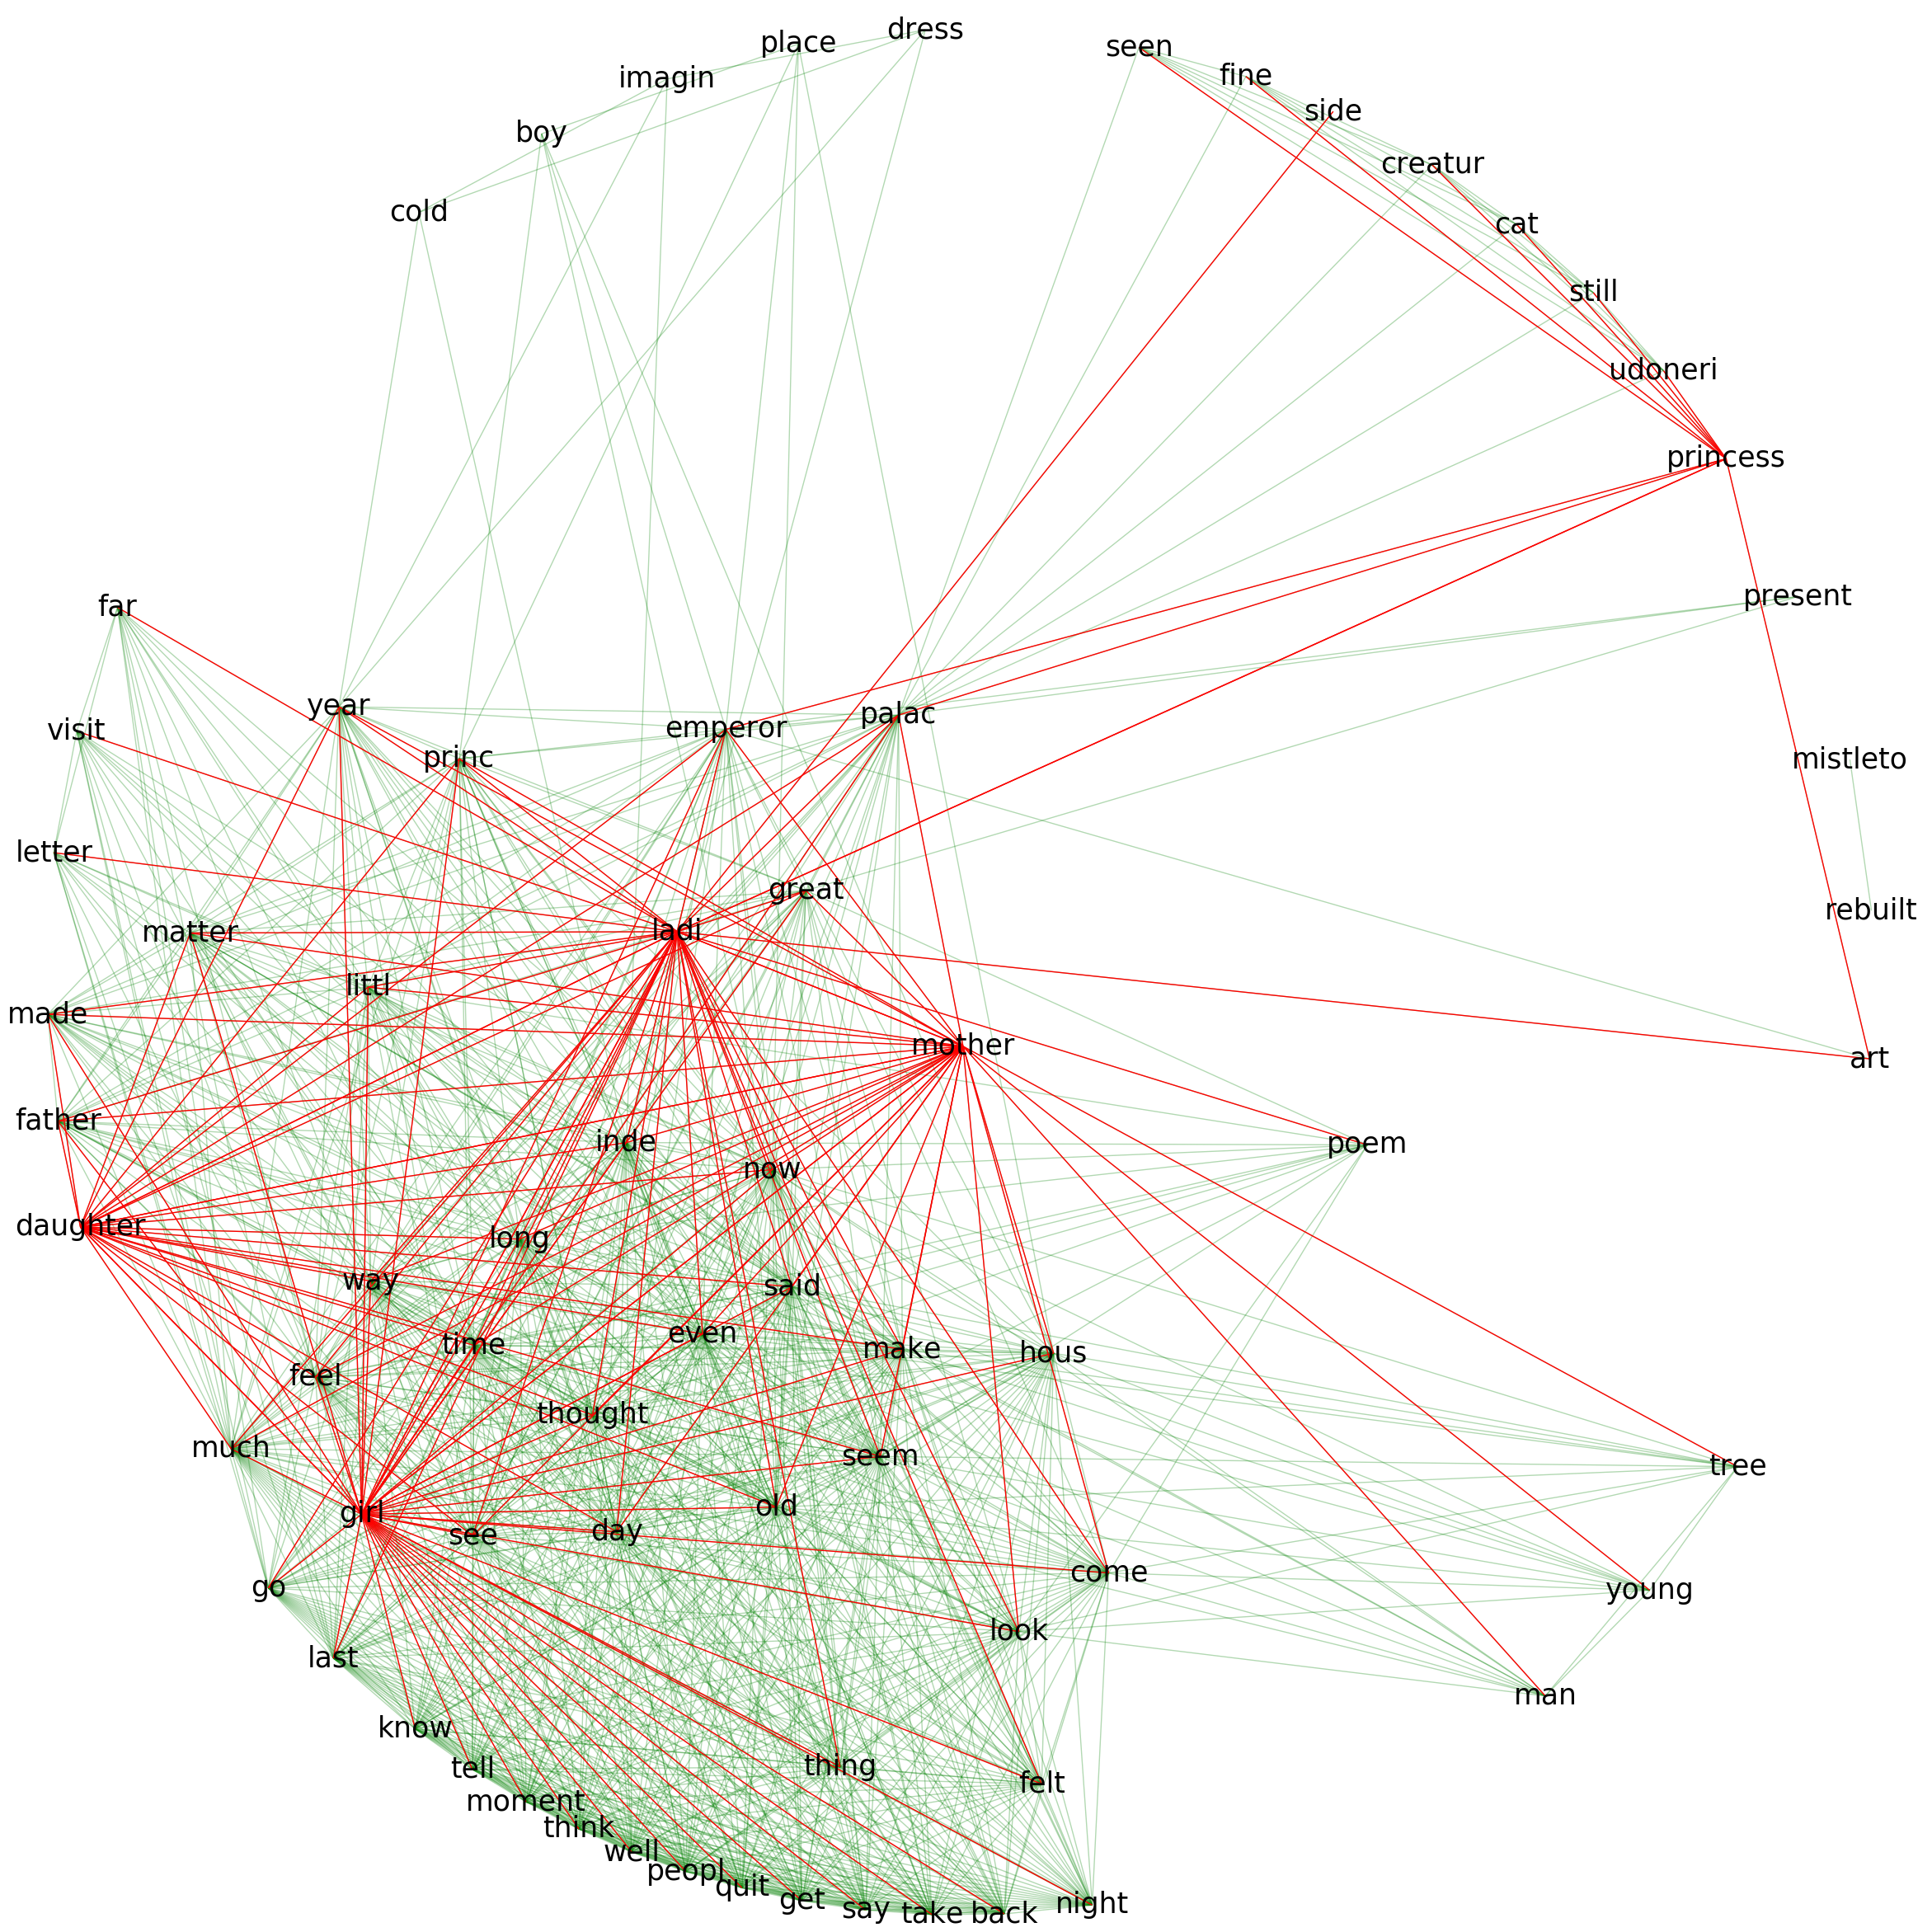
\includegraphics[width=3in]{waley-complete.png}
			\caption{Waley}
		\end{subfigure}		
	\end{subfigure}
	\caption{Thematic Structure: Female-Associated Connections in Red}
	\label{full-networks}
\end{figure}

\begin{figure}
	\begin{subfigure}{\linewidth}
		\begin{subfigure}{.5\linewidth}
	  		\includegraphics[width=3in]{washburn-complete.png}\hfill
	  		\caption{Washburn}
	  	\end{subfigure}
	  	\begin{subfigure}{.5\linewidth}
	  		\includegraphics[width=3in]{tyler-complete.png}
	  		\caption{Tyler}
	  	\end{subfigure}
	\end{subfigure}\par\medskip
	\begin{subfigure}{\linewidth}
		\begin{subfigure}{.5\linewidth}	
			\includegraphics[width=3in]{seidensticker-complete.png}\hfill	
			\caption{Seidensticker}
		\end{subfigure}
		\begin{subfigure}{.5\linewidth}			
			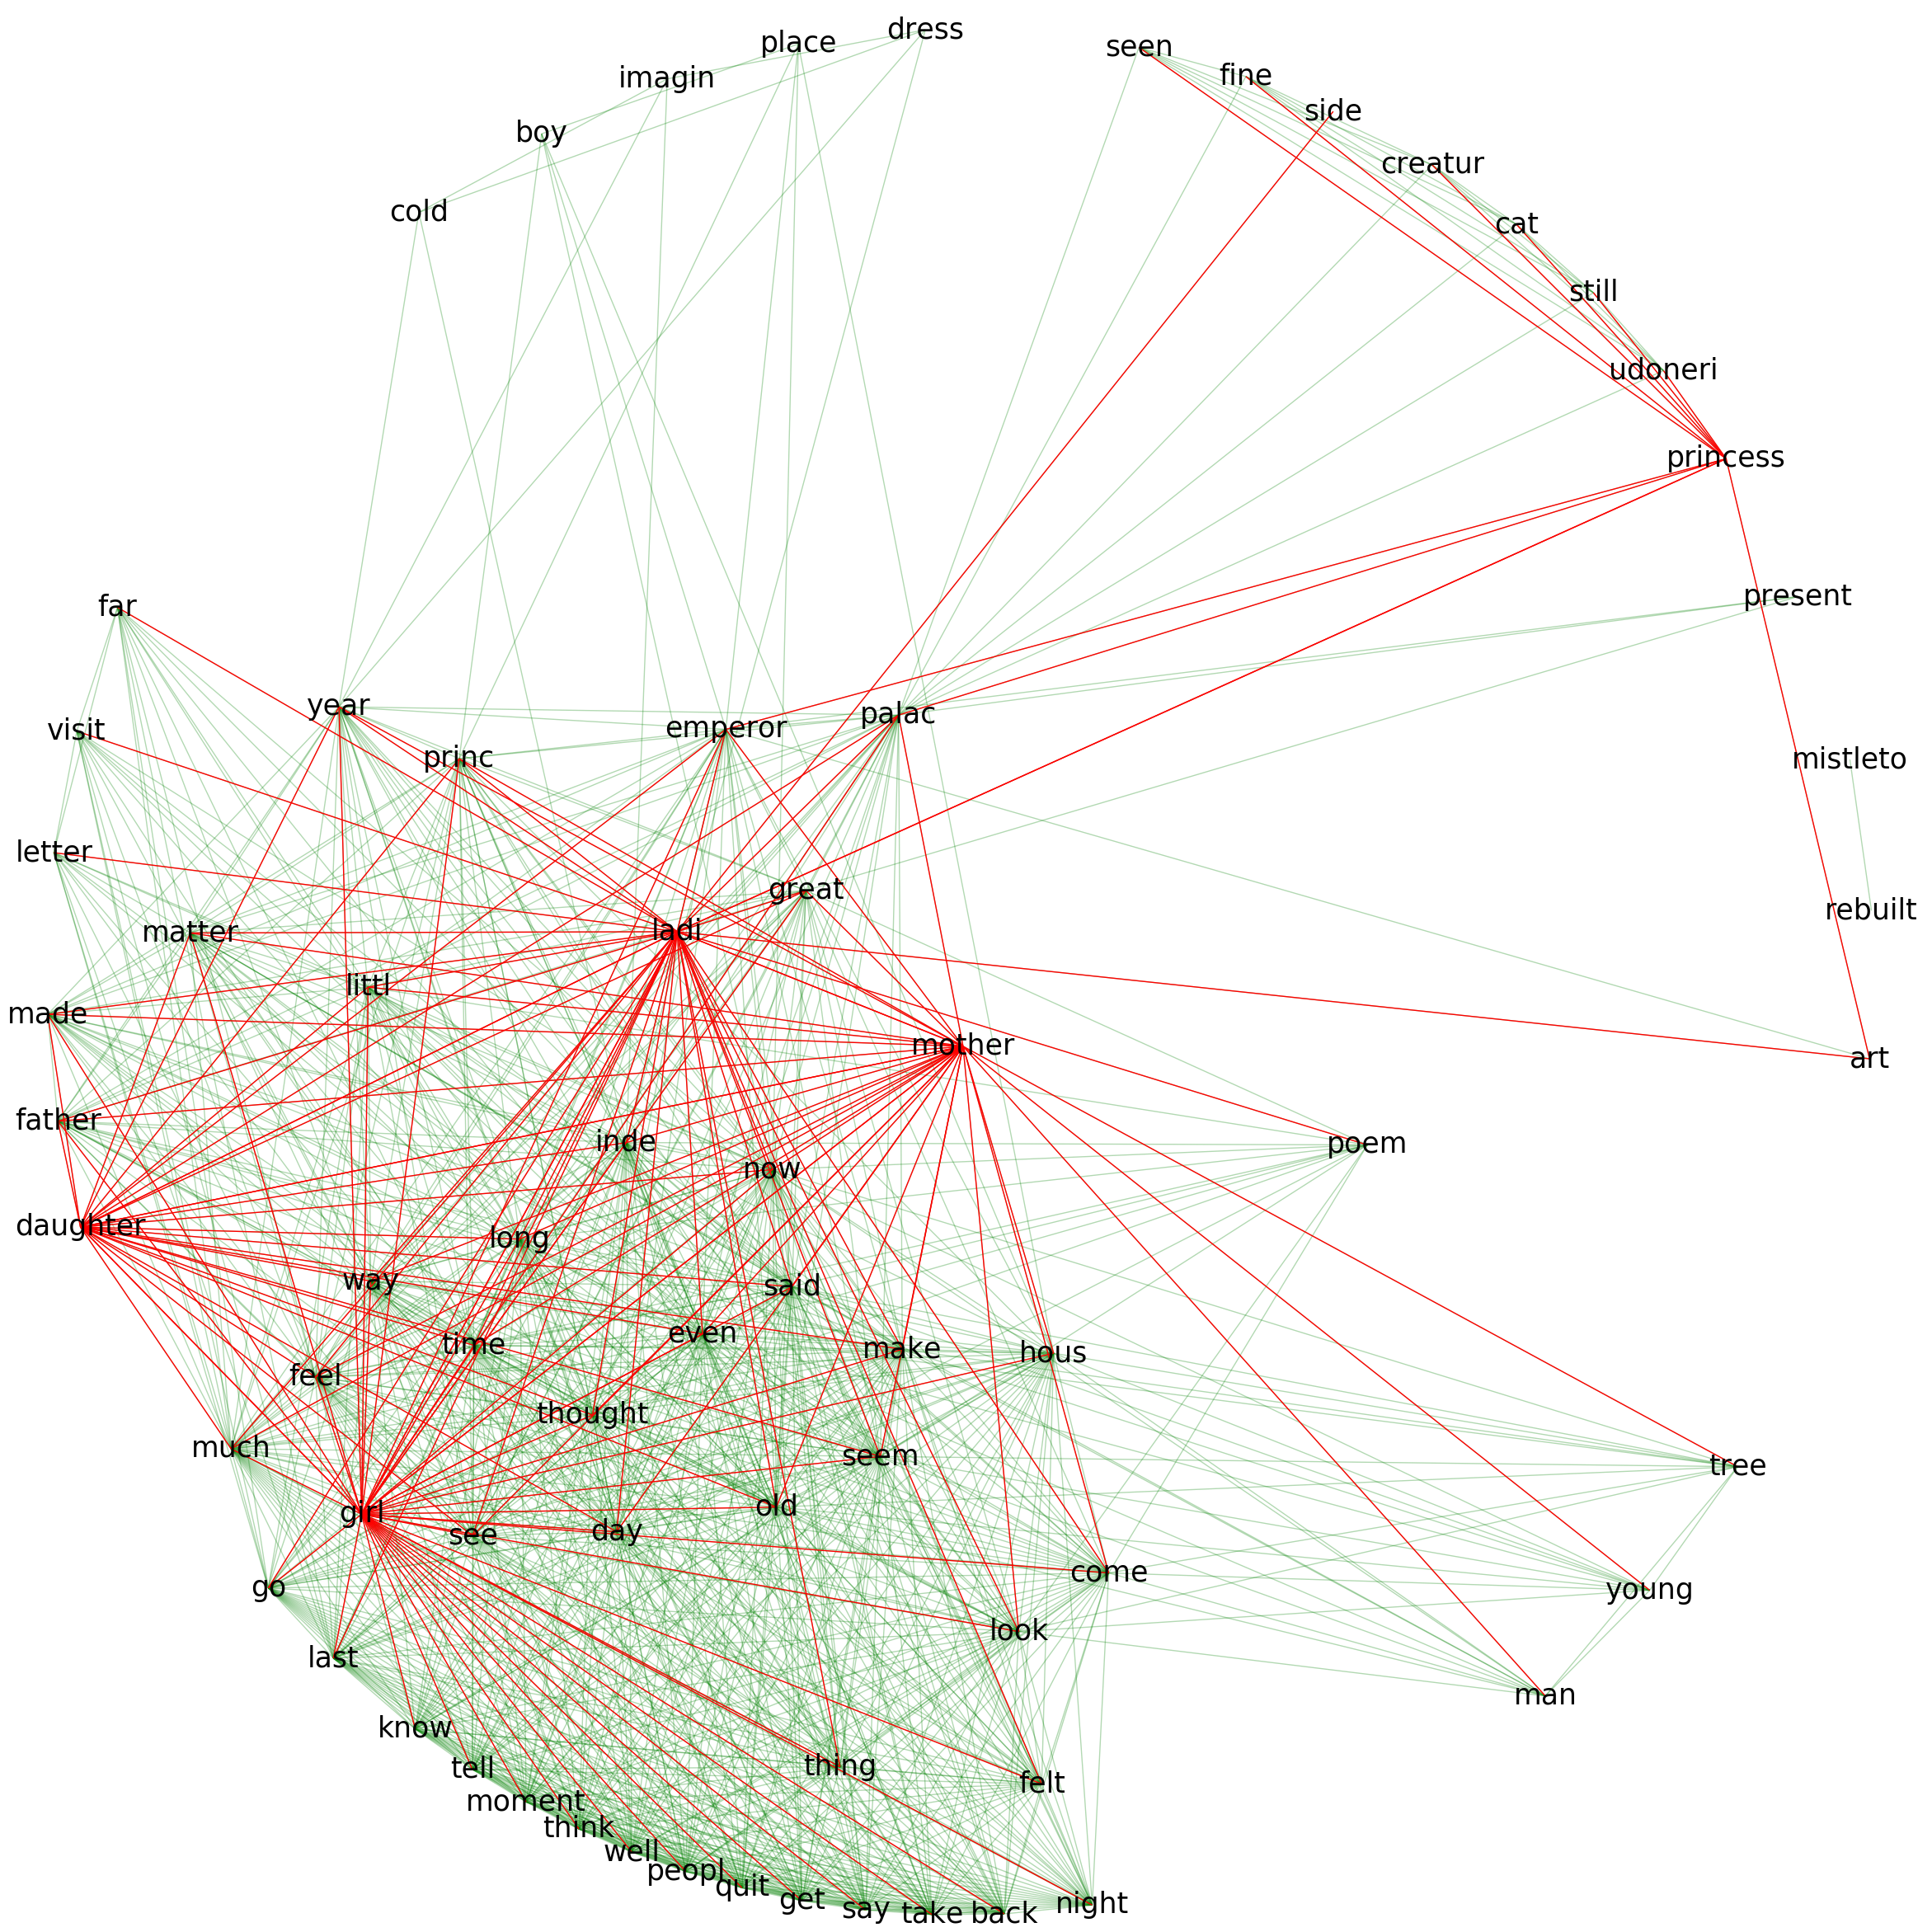
\includegraphics[width=3in]{waley-complete.png}
			\caption{Waley}
		\end{subfigure}		
	\end{subfigure}
	\caption{Thematic Structures Without Women}
	\label{full-networks}
\end{figure}


%  \caption{Washburn's Thematic Structure: Female-Associated Connections in Red}
%  
%\end{figure}
%
%\begin{figure}
%    \caption{Tyler's Thematic Structure: Female-Associated Connections in Red}
%  \label{fig:tyler-full}
%\end{figure}
%
%\begin{figure}
%  
%  \caption{Seidensticker's Thematic Structure: Female-Associated Connections in Red}
%  \label{fig:seidensticker-full}
%\end{figure}
%
%\begin{figure}
%  
%  \caption{Waley's Thematic Structure: Female-Associated Connections in Red}
%  \label{fig:waley-full}
%\end{figure}
%
\begin{figure}
  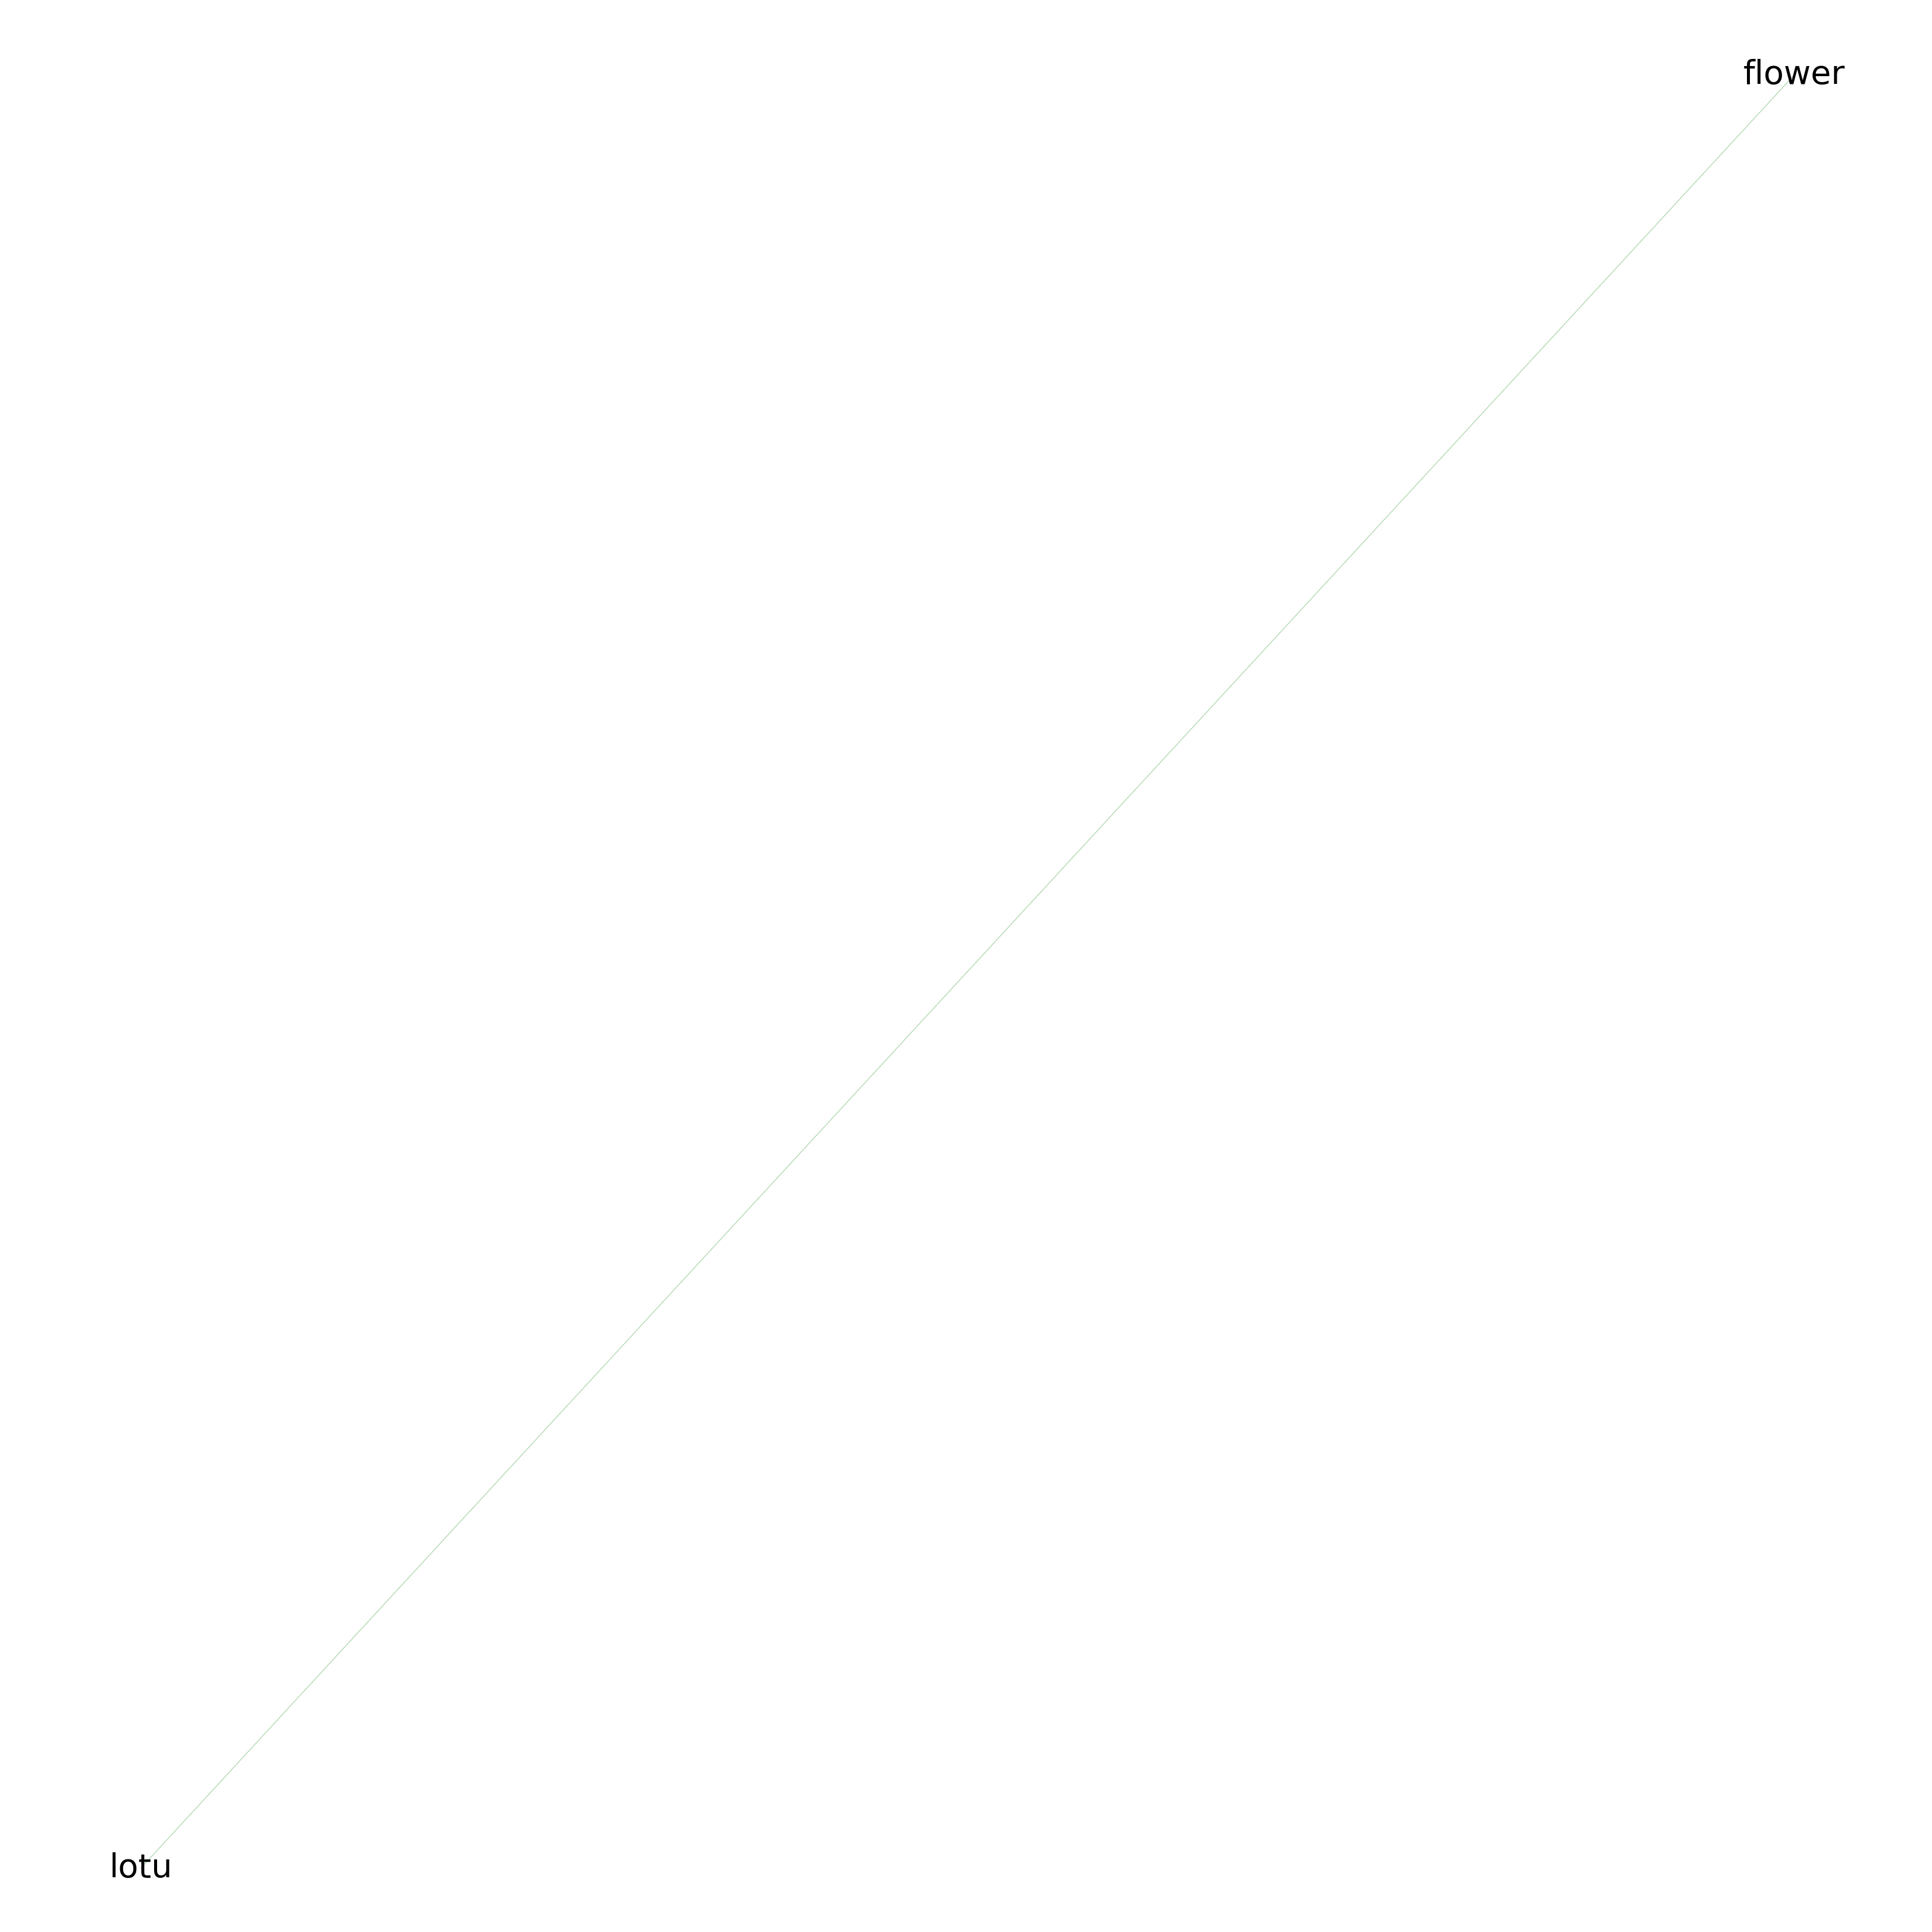
\includegraphics[width= 3in]{washburn-no-womenwords.png}
  \caption{Washburn Without Women-Associated Words}
  \label{fig:washburn-no-womenwords}
\end{figure}

\begin{figure}
  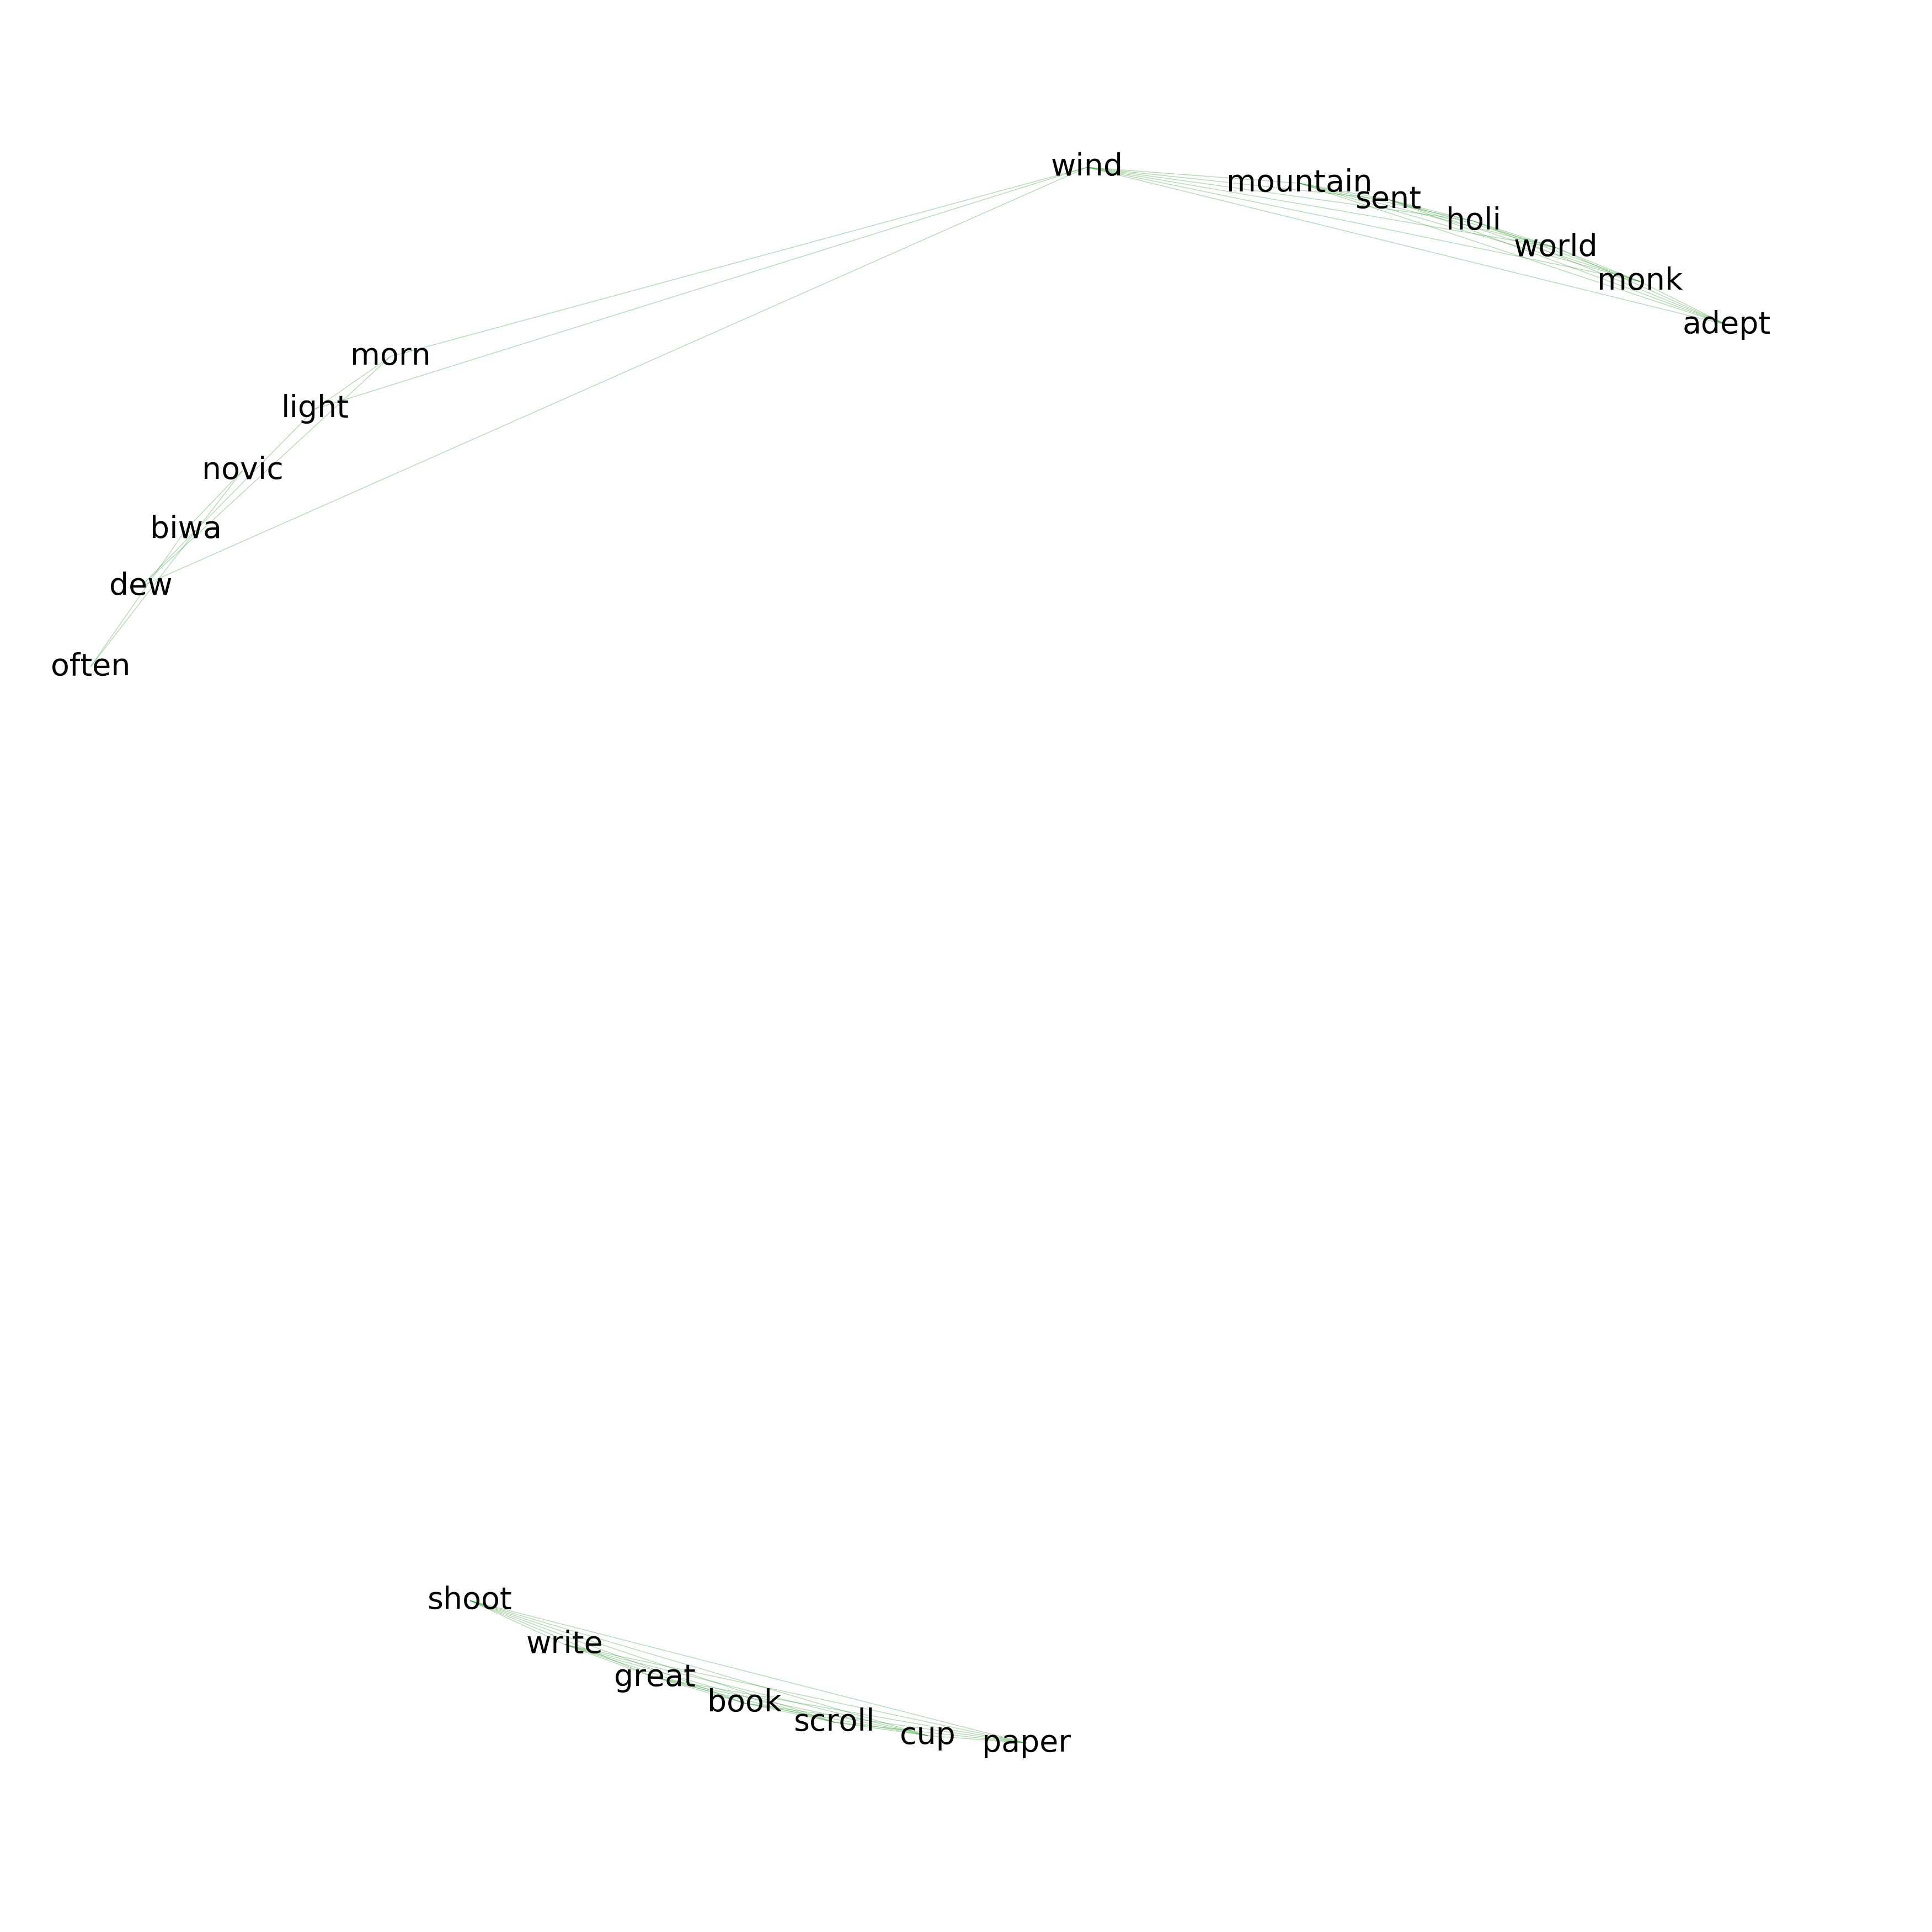
\includegraphics[width= 3in]{tyler-no-womenwords.png}
  \caption{Tyler Without Women-Associated Words}
  \label{fig:washburn-no-womenwords}
\end{figure}

\begin{figure}
  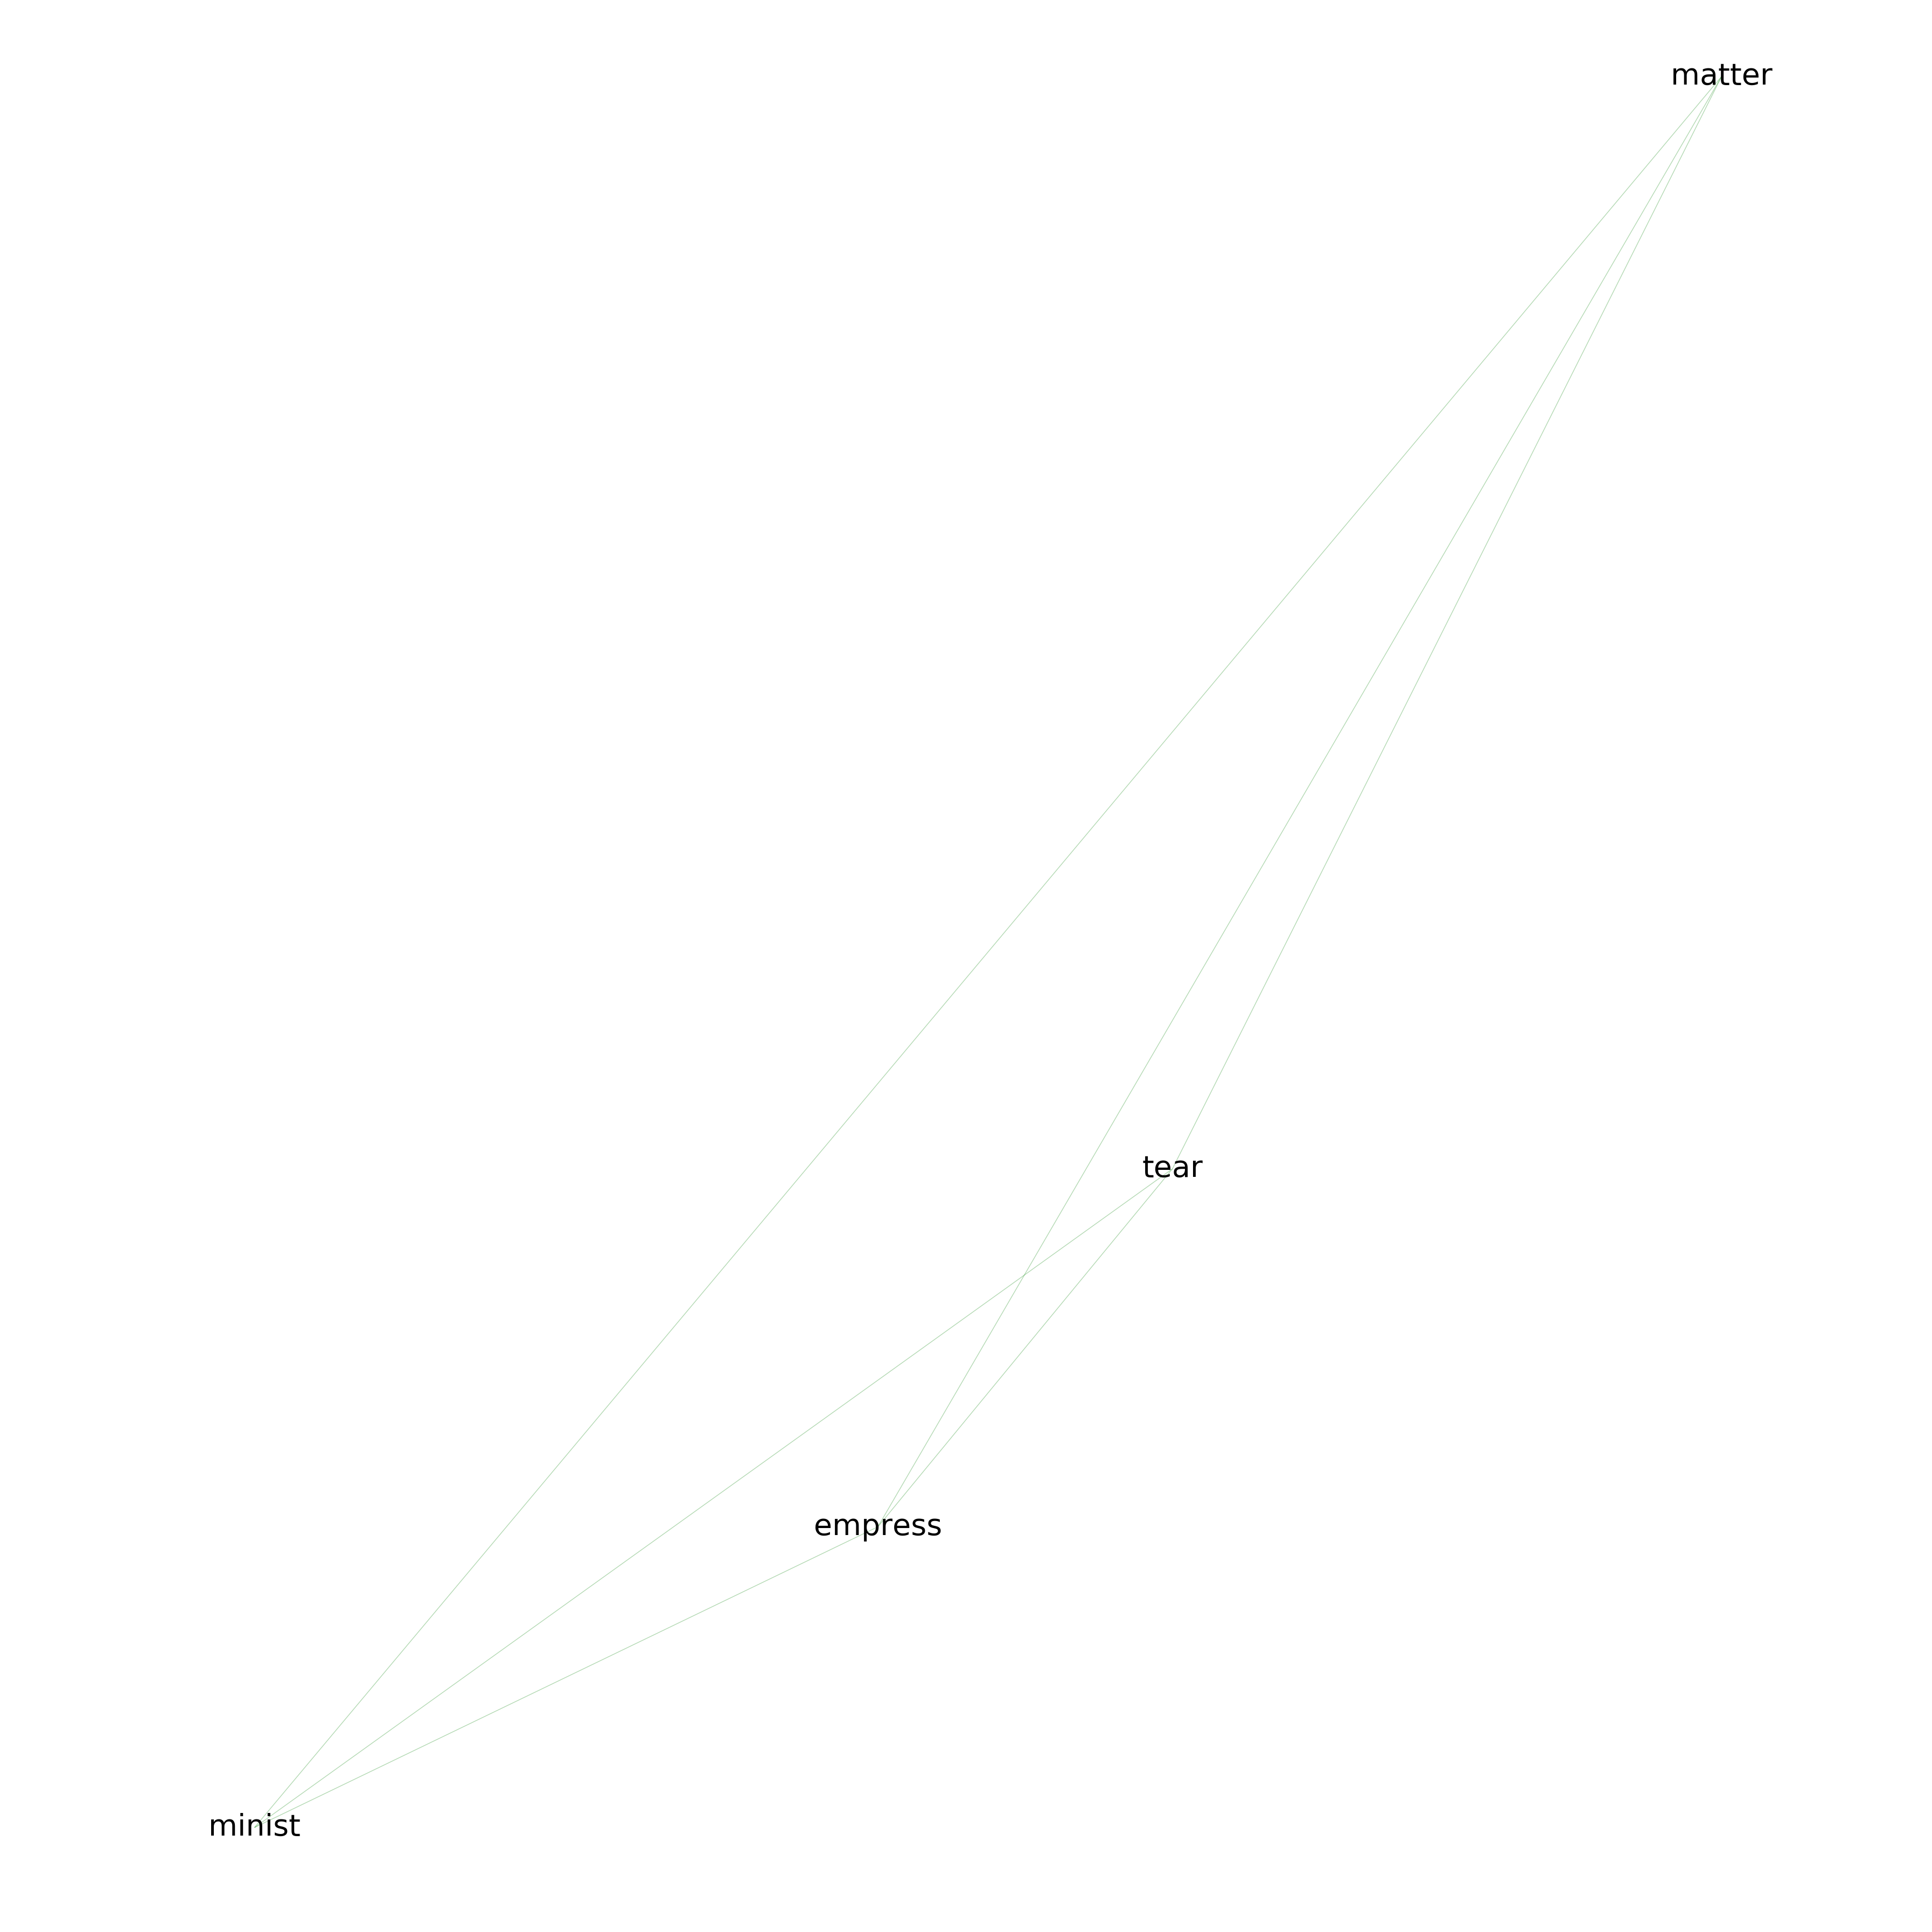
\includegraphics[width= 3in]{seidensticker-no-womenwords.png}
  \caption{Seidensticker Without Women-Associated Words}
  \label{fig:washburn-no-womenwords}
\end{figure}


\begin{figure}
  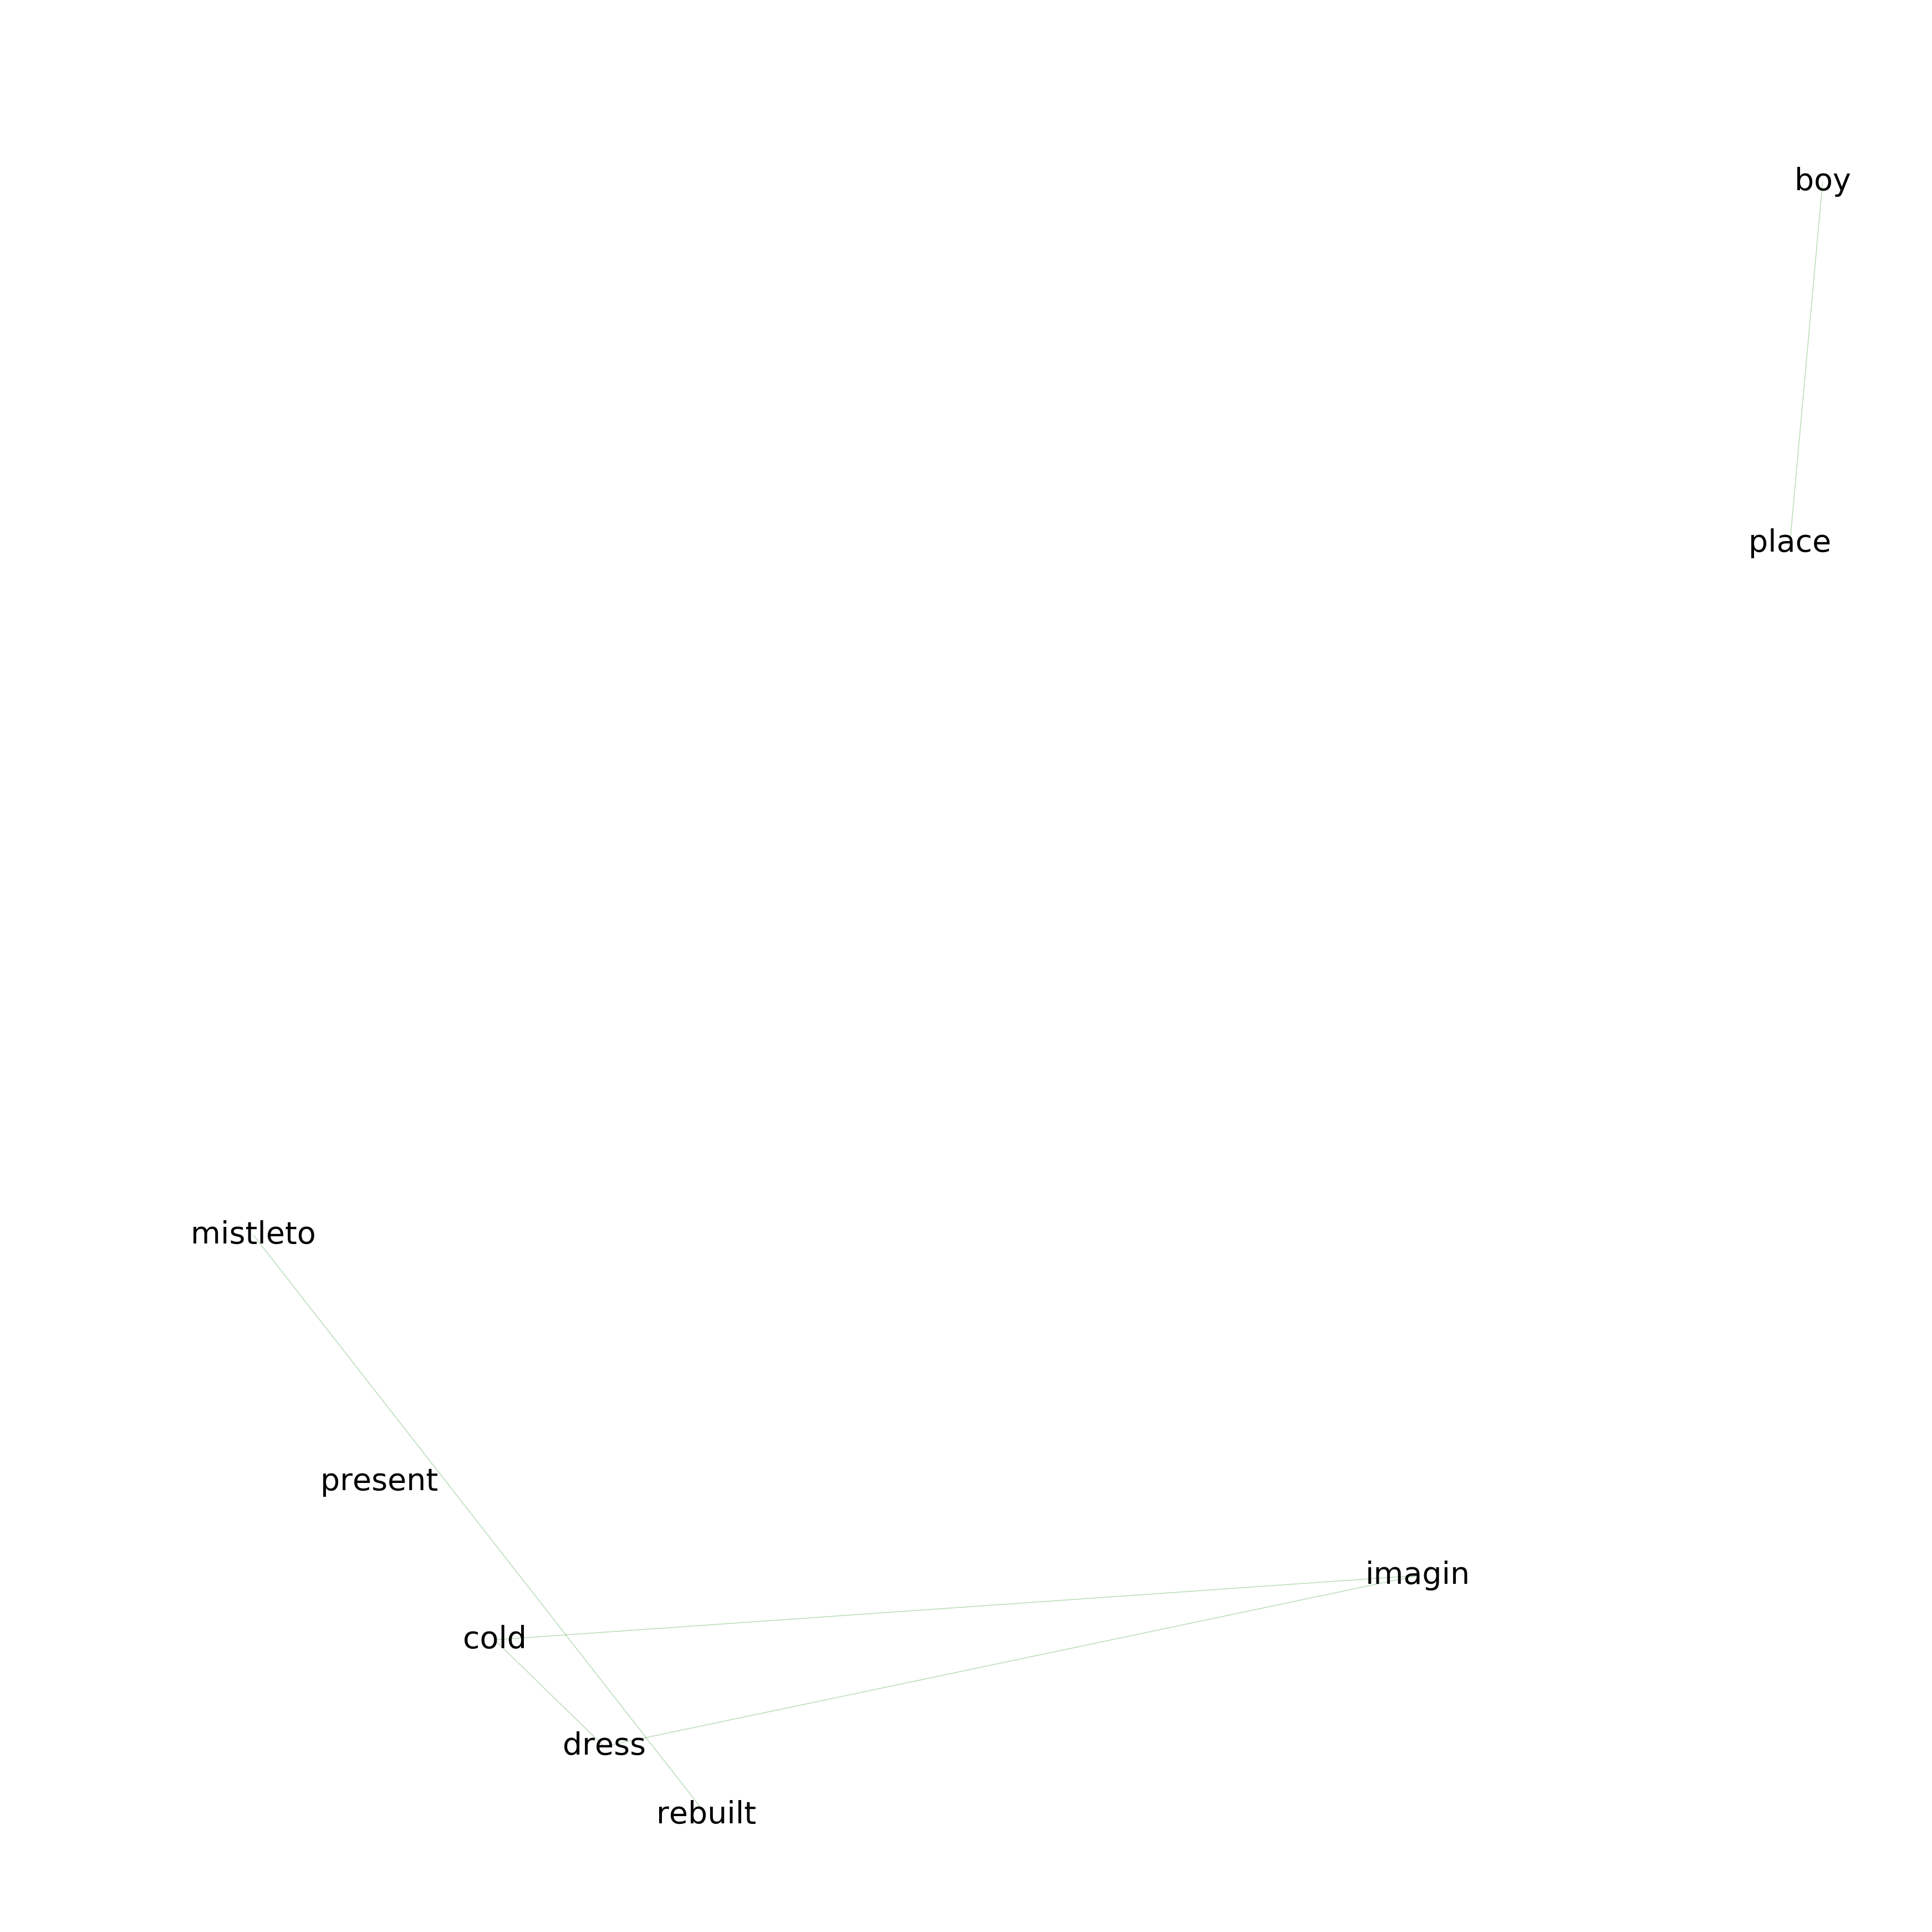
\includegraphics[width= 3in]{waley-no-womenwords.png}
  \caption{Waley Without Women-Associated Words}
  \label{fig:washburn-no-womenwords}
\end{figure}


An analysis of each thematic network without women reveals the centrality of their role in all four translations of the Genji: the structure of Washburn collapses entirely, leaving a virtually nonexistent graph, (See Figure \ref{fig:washburn-no-womenwords}), Seidensticker 

The most intriguing changes, however, are when we remove individual female words rather than all female words in their entirety. Removal of the word 'mother' has different effects on each network, reducing Seidensticker's to a notably more romantic, sentimental, and courtship-heavy structure. In Waley's case, removal of the word "mother" results in 

Removing feeling and thinking words, specifically 'feel', 'felt', 'think', 'thought', 'emot', removes all mention of females from Seidensticker's network. 

Removing duty and palace-related words reduces the female network of Tyler almost exclusively to independent women-words, and removal of feeling-thinking words reduces the network almost entirely to male-independent women.
\begin{workscited}

\bibent Jockers, M. L..\booktitle{Macroanalysis: Digital Methods and Literary History}. Champaign: University of Illinois Press, 2013. Project MUSE.

\bibent Rhody, Lisa M. ``Topic Modeling and Figurative Language.'' \booktitle{Journal of Digital Humanities}, vol. 2, no. 1, 2012, pp. 19---38.

\bibent Henitiuk, Valerie. ``Going to Bed with Waley: How Murasaki Shikibu does and does not become world literature.'' \booktitle{Comparative Literature Studies}, vol. 45, no. 1, 2008, pp. 40---61., www.jstor.org/stable/25659632.

\bibent Meeks, Elijah. ''Using Word Clouds for Topic Modeling Results.'' \booktitle{Digital Humanities Specialist}. N.p., 15 Aug. 2012. Web. 16 Apr. 2017. <https://dhs.stanford.edu/algorithmic-literacy/using-word-clouds-for-topic-modeling-results/>.

\bibent Shikibu, Murasaki, and Dennis C. Washburn. \booktitle{The Tale of Genji}. New York: W.W. Norton, 2015. Amazon.com. Web.

\bibent Shikibu, Murasaki, and Arthur Waley. \booktitle{The Tale of Genji}. Boston and New York: Houghton Mifflin, 1925. Amazon.com. Web.

\bibent Murasaki Shikibu B. ''University of Oxford Text Archive.'' [OTA] \booktitle{The Tale of Genji} [Electronic Resource]. Trans. Edward G. Seidensticker. N.p., n.d. Web. 16 Apr. 2017. <http://ota.ox.ac.uk/desc/2245>.

\bibent Murakami, Janel R. Goodman. ''Metonymy in The Tale of Genji: An Analysis of Translation Strategies.'' \booktitle{Arizona Working Papers in SLA and Teaching 20} (2013): 55-75.	

\bibent Moretti, Franco. ``Network Theory, Plot Analysis.'' \booktitle{Distant Reading}. London: Verso, 2015. N. pag. Print.

\end{workscited}



\end{spacing}
\end{flushleft}
\end{document}
